\documentclass[english,11pt,a4paper]{article}

\usepackage{pgfplots}
\pgfplotsset{compat=newest}
%% the following commands are sometimes needed
\usetikzlibrary{plotmarks}
\usepackage{grffile}

\usepackage{latexsym}
\usepackage{babel}
% %\usepackage{rotating}
\usepackage{subfig}
%\usepackage{multibbl}
%\usepackage{calc}
%\usepackage{lastpage}
\usepackage{amsmath,epsfig,amssymb,amsbsy, amsthm}
%\usepackage{euproposal}
\usepackage{multirow}
%\usepackage{natbib}
%\usepackage{multibib}
%\usepackage{fancybox}
\usepackage{nicefrac}
%\usepackage[table]{xcolor}
%\usepackage[right]{eurosym}



\usepackage[bordercolor=white,backgroundcolor=gray!30,linecolor=black,colorinlistoftodos]{todonotes}

%\usepackage[T1]{fontenc}

\usepackage{wrapfig,graphicx}
\usepackage{url}
%\usepackage{titlesec}

\usepackage{color}
\usepackage{colortbl}

\newcommand{\todobase}[3]{\todo[color=#3,inline]{#2}}

\newcommand{\jl}[1]{\todobase{J}{#1}{yellow}}
\newcommand{\tmo}[1]{\todobase{J}{#1}{pink}}
\newcommand{\mm}[1]{\todobase{J}{#1}{cyan}}

\renewcommand{\baselinestretch}{1.2} 

\newcommand\dimOmega{d}
\newcommand{\ngradients}{m}
\newcommand{\mfindex}{k} %k
\newcommand{\unarycost}{s}
\newcommand{\mfweights}{b}
\newcommand{\bitem}{\begin{itemize}}
\newcommand{\eitem}{\end{itemize}}
\newcommand{\mc}[1]{\mathcal{#1}}
\newcommand{\mb}[1]{\mathbb{#1}}
\newcommand{\R}{\mathbb{R}}
\newcommand{\B}{\mathbb{B}}
\newcommand{\U}{\mathbb{U}}
\newcommand{\E}{\mathbb{E}}
\newcommand{\Q}{\mathbb{Q}}
\newcommand{\Z}{\mathbb{Z}}
\newcommand{\PP}{\mathbb{P}}
\newcommand{\bpm}{\begin{pmatrix}}      
\newcommand{\epm}{\end{pmatrix}}
\newcommand{\T}{\top}
\newcommand{\tr}{\mathsf{tr}}
\newcommand{\ol}[1]{\overline{#1}}      
\newcommand{\la}{\langle}
\newcommand{\ra}{\rangle}
\newcommand{\si}{\sigma}
\newcommand{\mrm}[1]{\mathrm{#1}}
\newcommand{\msf}[1]{\mathsf{#1}}
\newcommand{\Diag}{\mathrsf{Diag}}
\newcommand{\row}[2]{{#1}_{#2,\bullet}}
\newcommand{\col}[2]{{#1}_{\bullet,#2}}
\newcommand{\veps}{\varepsilon}
\newcommand{\toset}{\rightrightarrows}
\newcommand{\w}{\omega}
\newcommand{\gdw}{\Leftrightarrow}
\newcommand{\vphi}{\varphi}
\newcommand{\tmop}[1]{\ensuremath{\operatorname{#1}}}
\newcommand{\norm}[1]{\Vert #1 \Vert}
\newcommand{\normc}[1]{| #1 |}
\newcommand{\bbR}{\mathbb{R}}
\newcommand{\bbRext}{\mathbb{R} \cup \{ \infty \} }
\newcommand{\bbN}{\mathbb{N}}
\providecommand{\iprod}[2]{\langle#1,#2\rangle}


\newcommand{\bi}{\begin{itemize}}
\newcommand{\ei}{\end{itemize}}
\newcommand{\HH}{\mathcal{H}}
\newcommand{\MM}{\mathcal{M}}

\newcommand{\DD}{\mathcal{D}}
\newcommand{\JJ}{\mathcal{J}}
\newcommand{\Ss}{\mathcal{S}}

\newcommand{\reps}{\rho_{\veps}}
\newcommand{\geqs}{\geqslant}
\newcommand{\leqs}{\leqslant}


%\newcommand{\cref}[1]{ [{#1}]}
\newcommand{\cref}[1]{ {\tiny[{#1}]}}
%\newcommand{\tm}[1]{[#1] }
\newcommand{\tm}[1]{}

\newcommand{\VI}{\mathsf{VI}}
\newcommand{\SOL}{\mathsf{SOL}}
\newcommand{\graph}{\mathsf{gph}}
\newcommand{\dom}{\mathsf{dom}}
\newcommand{\conv}{\mathsf{conv}}
\newcommand{\rint}{\mathsf{rint}}
\newcommand{\bd}{\mathsf{bd}}
\newcommand{\rge}{\mathsf{rge}}
\newcommand{\epi}{\mathsf{epi}}
\newcommand{\lev}{\mathsf{lev}}
\newcommand{\argmin}{\mathsf{argmin}}
\newcommand{\argmax}{\mathsf{argmax}}

\newcommand{\detail}{\ding{43} \structure{Detail}}

\newcommand{\fr}[3][]{\frame{\frametitle{#2}\begin{textblock*}{6cm}(12cm,1.5cm)\rotatebox{90}{\parbox{7cm}{\scriptsize\structure{#1}}}\end{textblock*}\bi #3 \ei}}
\newcommand{\frb}[3][]{\frame{\frametitle{#2}\begin{textblock*}{6cm}(12cm,1.5cm)\rotatebox{90}{\parbox{7cm}{\scriptsize\structure{#1}}}\end{textblock*}#3}}
\newcommand{\tmemtitle}{\textbf}

\newcommand{\mathbbm}{\mathbb}
\newcommand{\C}{\mathcal{C}}
\newcommand{\D}{\mathcal{D}}
\newcommand{\Rn}{\mathbb{R}^n}
\newcommand{\Rm}{\mathbb{R}^m}
\newcommand{\Rmxn}{\mathbb{R}^{m \times n}}
\newcommand{\Rd}{\mathbb{R}^d}
\newcommand{\Rl}{\mathbb{R}^L}
\newcommand{\beq}{\begin{equation}}
\newcommand{\eeq}{\end{equation}}
\newcommand{\beqa}{\begin{eqnarray}}
\newcommand{\eeqa}{\end{eqnarray}}
\newcommand{\bc}{\begin{center}}
\newcommand{\ec}{\end{center}}
\newcommand{\lcb}{\left\{}
\newcommand{\rcb}{\right\}}
\newcommand{\lbr}{\left(}
\newcommand{\rbr}{\right)}
\newcommand{\seq}{\subseteq}
\newcommand{\PC}{\Pi_{\C}}
\newcommand{\PD}{\Pi_{\D}}
\newcommand{\assign}{:=}
\newcommand{\Om}{\Omega}
\newcommand{\BV}{\tmop{BV}}
\newcommand{\SBV}{\tmop{SBV}}
\newcommand{\Ccinf}{C_c^{\infty}}
\newcommand{\Dloc}{\D_{\tmop{loc}}}
\newcommand{\Hausd}{\mathcal{H}}
\newcommand{\tmtextbf}[1]{{\bfseries{#1}}}
\newcommand{\tmtextit}[1]{{\itshape{#1}}}
\newcommand{\tmem}[1]{{\em #1\/}}
%\newcommand{\subs}[1]{\smallskip\noindent\textbf{#1.} }
\newcommand{\subs}[1]{\medskip\noindent\textbf{#1.} }
%\newcommand{\subs}[1]{\noindent\textbf{#1.} }
%\newcommand{\subs}[1]{\paragraph{#1.} }

\newcommand{\wi}{.1\columnwidth}

\newcommand \M   {{\mathcal{M}}}                     % manifold

\newcommand \Sone       {{{\Ss}^1}}                         % S^1
\newcommand \TVS        {{TV_\Sone}}                        % TV_{S^1}
\newcommand \TVM        {{TV_\M}}                           % TV_{S^1}
\newcommand \Stwo       {{{\Ss}^2}}                         % S^1
\newcommand \TVStwo     {{TV_\Stwo}}                        % TV_{S^1}
\newcommand \TVSg       {{TV_\Sone^g}}                      % TV_{S^1}^g
\newcommand \TV         {{TV}}                              % TV
\newcommand{\dx}        {\,dx}
\newcommand \Su         {{S_u}}                             % subset
% of Omega w 
\newcommand \omegaDim   {{m}}                               % image domain dimension
\newcommand \dH         {{d\;\!\mathcal{H}^{\omegaDim-1}}}  % Hausdorff measure
\newcommand{\Div}{\tmop{Div}}


%\arrayrulecolor{black} % green tables otherwise
%\renewcommand{\familydefault}{\sfdefault}
%\usepackage{arial}

\newcommand{\fc}{^{\ast}}
\newcommand{\fcc}{^{\ast\ast}}
\newcommand{\ow}{\text{otherwise}}

\newcommand{\RL}{\R^L}
\newcommand{\Rb}{\bar{\R}}

%\newtheorem{thm}{Theorem}[section]
%\newtheorem{prop}[thm]{Proposition}

\newtheorem{lem}{Lemma}
\newtheorem{prop}{Proposition}
\newtheorem{cor}{Corollary}
\newtheorem{rem}{Remark}

\newcommand{\dat}{\boldsymbol{\rho}}
\newcommand{\dats}{\boldsymbol{\sigma}}
\newcommand{\reg}{\boldsymbol{\Phi}}
\newcommand{\Gr}{\mathbf{1}}
\newcommand{\ul}{\boldsymbol{u}}
\newcommand{\el}{\boldsymbol{e}}
\newcommand{\vl}{\boldsymbol{v}}
\newcommand{\Vl}{\boldsymbol{V}}
\newcommand{\gl}{\boldsymbol{g}}
\newcommand{\pl}{\boldsymbol{p}}
\newcommand{\ql}{\boldsymbol{q}}
\newcommand*\Bell{\ensuremath{\boldsymbol\ell}}
\newcommand*\Bgamma{\ensuremath{\boldsymbol\gamma}}

\newcommand*{\vertbar}{\rule[-1ex]{0.5pt}{2.5ex}}

\newcommand\inner[2]{\langle #1, #2 \rangle}

\usepackage{a4wide}
\usepackage{tikz}

\title{Ideas for Splitting Deep Networks}
\author{}
\usepackage{amsmath,epsfig,amssymb,amsbsy}

\begin{document}
\maketitle

\section{Objective function}

The aim is to solve a supervised regression or classification problem involving a highly nested objective function. A mapping $f(x)$ from the inputs $x$ to the corresponding outputs $y$ based on $N$ training samples $(x_n, y_n)$ should be learned. The loss function can be formulated as

\begin{equation}
E(W) = \frac{1}{N} \sum_{i=1}^{N} L(f(W;x_i);y_i)
\label{eq:1}
\end{equation}

with some appropriate error measure $L(y_t;y)$. This error measure can for example be the squared l2-loss $L(y_t;y) = \frac{1}{2} \| y_t - y \|^2_2$. The function $f(W;x) = W_{K+1}h(W_Kh(\dots h(W_1x))$ is a nested K-layer mapping as it is usual in neural networks where $W$ are the weight matrices $W_1,\dots,W_{K+1}$ which do not need to have the same size. The nonlinear activation function $h(x)$ is applied element-wise and can also be non-differential. Examples are the sigmoid function $h(x) = 1/(1 + e^{-x})$ or the ReLU $h(x) = \mathrm{max}(0, x)$.

\section{Solution concept}

In the following, we stack all input samples into the matrix $x$ where each column is one sample point. Similarly, the target variables are stacked into the matrix $y$. The error function $L$ now operates on matrices. This formulation is equal to the formulation above, however, the layers now operate on all the data simultaneously. Additionally, without loss of generality we consider a 2-layer neural network mapping $f(W;x) = W_3h(W_2h(W_1x))$ with a linear mapping to the output variables. The unconstrained optimization problem can then be written as

\begin{equation}
	\begin{aligned}
		& \underset{\{W_i\}}{\text{minimize}}
		& & L(W_3h(W_2h(W_1x);y).
	\end{aligned}
\end{equation}

To split the nested objective function we decouple the weights and activation functions
by introducing additional variables and adding the appropriate constraints. This reformulated problem is equal to the original problem and can be written as

\begin{equation}
	\begin{aligned}
		& \underset{\{W_i,a_i,z\}}{\text{minimize}}
		&& L(z;y). \\
		& \text{subject to}
		&&  a_1 = h(W_1x), \\
		&&& a_2 = h(W_2a_1), \\
		&&& z = W_3a_2
	\end{aligned}
\end{equation}

with the new variables $a_1, a_2, z$. The augmented Lagrangian of this equally constrained problem is

\begin{equation}
	\begin{aligned}
		\mathcal{L}(y,z,a,\lambda) = L(y,z) + 
		& \inner{\lambda_1}{h(W_1x)-a_1} + \rho/2 \| h(W_1x)-a_1 \|^2 + \\
		& \inner{\lambda_2}{h(W_2a_1)-a_2} + \rho/2 \| h(W_2a_1)-a_2 \|^2 + \\
		& \inner{\lambda_3}{W_3a_2-z} + \rho/2 \| W_3a_2-z \|^2.
	\end{aligned}
\end{equation}

with $a = (a_1,a_2)^T$, $\lambda = (\lambda_1, \lambda_2, \lambda_3)^T$ and $\rho \in \R$. For minimizing the objective we update the weights and constraint variables of subproblems in an alternating fashion using gradient descent. In each update step we only consider the variables of one constraint and fix all other terms of the augmented Lagrangian. This results in one subproblem $\mathcal{H}_i$ for each constraint.

\begin{equation}
	\begin{aligned}
		\mathcal{H}_1(W_1,a_1,\lambda_1) &= && \inner{\lambda_1}{h(W_1x)-a_1} + \rho/2 \| h(W_1x)-a_1 \|^2 + \\
			& && \inner{\lambda_2}{h(W_2a_1)-a_2} + \rho/2 \| h(W_2a_1)-a_2 \|^2 \\
		\mathcal{H}_2(W_2,a_1,a_2,\lambda_2) &= && \inner{\lambda_2}{h(W_2a_1)-a_2} + \rho/2 \| h(W_2a_1)-a_2 \|^2 + \\
			& && \inner{\lambda_1}{h(W_1x)-a_1} + \rho/2 \| h(W_1x)-a_1 \|^2 + \\
			& && \inner{\lambda_3}{W_3a_2-z} + \rho/2 \| W_3a_2-z \|^2 \\
		\mathcal{H}_3(W_3,a_2,z,\lambda_3) &= && \inner{\lambda_3}{W_3a_2-z} + \rho/2 \| W_3a_2-z \|^2 + L(y,z) \\
			& && \inner{\lambda_2}{h(W_2a_1)-a_2} + \rho/2 \| h(W_2a_1)-a_2 \|^2 
	\end{aligned}
\end{equation}

We need to take special care of the first subproblem (constraint for the first layer) involving the input $x$ and the last subproblem (constraint for the last linear layer) involving the predicted variable $z$. For all others we consider the update scheme (here for $\mathcal{H}_2$)

\begin{equation}
	\begin{aligned}
		W_2^{t+1} &= W_2^t - \rho_1 \nabla_{W_2}(\mathcal{H}_2(W_2^t,a_1^t,a_2^t,\lambda_2^t)) \\
		a_1^{t+1} &= a_1^t - \rho_2 \nabla_{a_1}(\mathcal{H}_2(W_2^t,a_1^t,a_2^t,\lambda_2^t)) \\
		a_2^{t+1} &= a_2^t - \rho_3 \nabla_{a_2}(\mathcal{H}_2(W_2^{t+1},a_1^{t+1},a_2^t,\lambda_2^t)) \\
		\lambda_2^{t+1} &= \lambda_2^{t} + \rho (h(W_2^{t+1}a_1^{t+1})-a_2^{t+1})
	\end{aligned}
\end{equation}

which are gradient descent steps for the primal variables and gradient ascent steps for the dual variable $\lambda$. For $\mathcal{H}_1$ only $W_1$, $a_2$ and $\lambda_1$ need to be updated since $x$ is a constant. For the last subproblem $\mathcal{H}_{K+1}$ we need to add $\nabla_zL(y,z)$ to the gradient with respect to $z$.

\section{Appendix}

\subsection{Notation}

For a matrix $X$, $X_{ij}$ selects the element in row $i$ and column $j$. If only one index is present, depending on the subscript a matrix row or column is select. In this case, $X_i$ is row $i$, $X_j$ is column $j$.

\subsection{Energy gradients}

For the update steps we need the gradient of the terms $f(W,x,a,\lambda) = \inner{\lambda}{h(Wx)-a}$ and $g(W,x,a) = (1/2) \| h(Wx) - a \|^2$ with respect to $W \in \R^{m \times n}$, $x \in \R^{n \times p}$, $a \in \R^{m \times p}$ and $\lambda \in \R^{m \times p}$. The function $h$ is applied element-wise. Note that for the inner product the matrices are vectorized. \\ \\
For the gradients we need the following intermediate results. For applying the chain-rule the derivatives of $h(Wx) = h \in \R^{m \times p}$ w.r.t $W$ and $x$ are required. Taking the derivative for each element the entries for the Jacobian are $\partial_{W_i}h_{ij} = h'(W_i x_j) x_j^T$. Similarly, for the derivatives w.r.t. $x$ we get $\partial_{x_j}h_{ij} = h'(W_i x_j) W_i^T $. Note that we can easily get a formulation for all matrix elements at once by the fact that for the Jacobians it holds that $J_{(f \circ g)} = J_f \cdot J_g$ and row $i$ of $J_f$ is $\nabla f_i$. This results in

\begin{equation}
	\begin{aligned}
		\partial_{W_i} f(W,x,a,\lambda) &= \sum_{j=1}^{p} \lambda_{ij} h'(W_i x_j) x_j^T \\
		\partial_{x_j} f(W,x,a,\lambda) &= \sum_{i=1}^{m} \lambda_{ij} h'(W_i x_j) W_i^T \\
		\partial_{\lambda} f(W,x,a,\lambda) &= h(W x) - a \\
		\partial_{a} f(W,x,a,\lambda) &= -\lambda
	\end{aligned}
\end{equation}

for the gradients of $f$. For $g$ the gradients are

\begin{equation}
	\begin{aligned}
		\partial_{W_i} g(W,x,a) &= \sum_{j=1}^{p} (h(W_i x_j) - a_{ij}) h'(W_i x_j) x_j^T \\
		\partial_{x_j} g(W,x,a) &= \sum_{i=1}^{m} (h(W_i x_j) - a_{ij}) h'(W_i x_j) W_i \\		
		\partial_{a} g(W,x,a) &= a - h(Wx). \\
	\end{aligned}
\end{equation}

Note that the expressions are in a format where we get a short formula. For calculating the matrix derivatives for all rows or for the complete matrix at once some matrix stacking is required which would result in a longer expression.

For the multi-class classification experiments we use the softmax error function $\ell(x)_i = \exp(x_i)/(\sum_{j=1}^{n} \exp(x_j))$ where $x \in \R^n$. The derivative of the softmax function is $\partial_{x_k} \ell(x)_i = \ell(x)_i (\delta_{ik} - \ell(x)_k)$.

\subsection{Backpropagation}

As baseline we train the loss function using gradient descent. To calculate the gradients $\nabla_{W}E(W)$ of the loss function $E(W)$ backpropagation is used. Starting from the definition of the loss function in equation \ref{eq:1} we can calculate the gradient for each sample separately by computing $\nabla_{W}L(f(W;x_i);y_i)$ and summing over all samples. In the following we consider $W_{jk}^l$ as the weight connecting neuron $k$ to neuron $j$ of layer $l$. The linearities in layer $l$ are written as $z^l = W^la^{l-1} + b^l$ operating on the activations $a^{l-1}$. The activations of layer $l$ are computed as $a^l = h(W^l a^{l-1} + b^l) = h(z^l)$ with activation function $h$. Additionally, we have used the explicit formulation with the bias being a separate variable. This could also be included in the weight matrix by augmenting the activation vector with one and augmenting the weight matrix with the bias vector as last column. Figure \ref{fig:backprop} shows the neural network model at a layer $l$. We introduce the convention of $E^l_a$ being the error function of layer $l$ given the activations and $E^l_z$ being the error function of layer $l$ given the linearities. This allows us to split the error function and use the chain rule for computing the derivatives. Using this formulation, the goal is to calculate $\nabla_{W}E(W,b)$ and $\nabla_{b}E(W,b)$. By fixing all remaining weights and biases and applying the chain rule we get

\begin{equation}
	\begin{aligned}
		\frac{\partial E(W_{jk}^l)}{\partial W_{jk}^l} &= 
		\frac{\partial E^l_a(a^l(z^l(W_{jk}^l)))}{\partial W_{jk}^l} =
		\frac{\partial E^l_a}{\partial a^l} \frac{\partial a^l}{\partial z^l} \frac{\partial z^l}{\partial W^l_{jk}} =
		\frac{\partial E^l_a}{\partial a^l_j} \frac{\partial a^l_j}{\partial z^l_j} \frac{\partial z^l_j}{\partial W^l_{jk}}, \\
		\frac{\partial E(b_j^l)}{\partial b_j^l} &=
		\frac{\partial E^l_a(a^l(z^l(b_j^l)))}{\partial b_j^l} =
		\frac{\partial E^l_a}{\partial a^l} \frac{\partial a^l}{\partial z^l} \frac{\partial z^l}{\partial b_j^l} =
		\frac{\partial E^l_a}{\partial a^l_j} \frac{\partial a^l_j}{\partial z^l_j} \frac{\partial z^l_j}{\partial b_j^l}.
	\end{aligned}
	\label{eq:backprop_chainrule}
\end{equation}

Note that $\frac{\partial z^l_i}{\partial W^l_{jk}} = 0$ and $\frac{\partial z^l_i}{\partial b_j^l} = 0$ for all $i \neq j$. We now introduce for each layer the error variable (row vector)

\begin{equation}
	\begin{aligned}
		\delta^l_j &= \frac{\partial E^l_a}{\partial a^l_j} \frac{\partial a^l_j}{\partial z^l_j} =
		\frac{\partial E^l_a}{\partial a^l_j} h'(z^l_j), \\
		\delta^l &= \frac{\partial E^l_a}{\partial a^l} \frac{\partial a^l}{\partial z^l} =
		\frac{\partial E^l_a}{\partial a^l} h'(z^l) = \frac{\partial E^l_a}{\partial a^l} \odot H'(z^l)^T
	\end{aligned}
\end{equation}

with $h'(z^l)$ being the Jacobian, $H'(z^l)$ the element-wise applied derivative of the activation function and $\odot$ the element-wise product. Note that the Jacobian is a diagonal matrix and we therefore can rewrite the equation using the Hadamard product. By expanding the first term we see that

\begin{equation}
	\begin{aligned}
		\frac{\partial E^l_a(a^l_j)}{\partial a^l_j} &= 
		\frac{\partial E^{l+1}_z(z^{l+1}(a^l_j))}{\partial a^l_j} = 
		\frac{\partial E^{l+1}_z}{\partial z^{l+1}} \frac{\partial z^{l+1}}{\partial a^l_j} = 
		\delta^{l+1}W^{l+1}_{:,j}, \\
		\frac{\partial E^l_a(a^l)}{\partial a^l} &= \delta^{l+1}W^{l+1}.
	\end{aligned}
\end{equation}

This shows that we can recursively compute the error variable $\delta^l$ starting from the last layer $L$ by

\begin{equation}
	\begin{aligned}
		\delta^l = \delta^{l+1}W^{l+1} h'(z^l) = \delta^{l+1}W^{l+1} \odot H'(z^l)^T.
	\end{aligned}
\end{equation}

\begin{figure}[t]
	\centering
	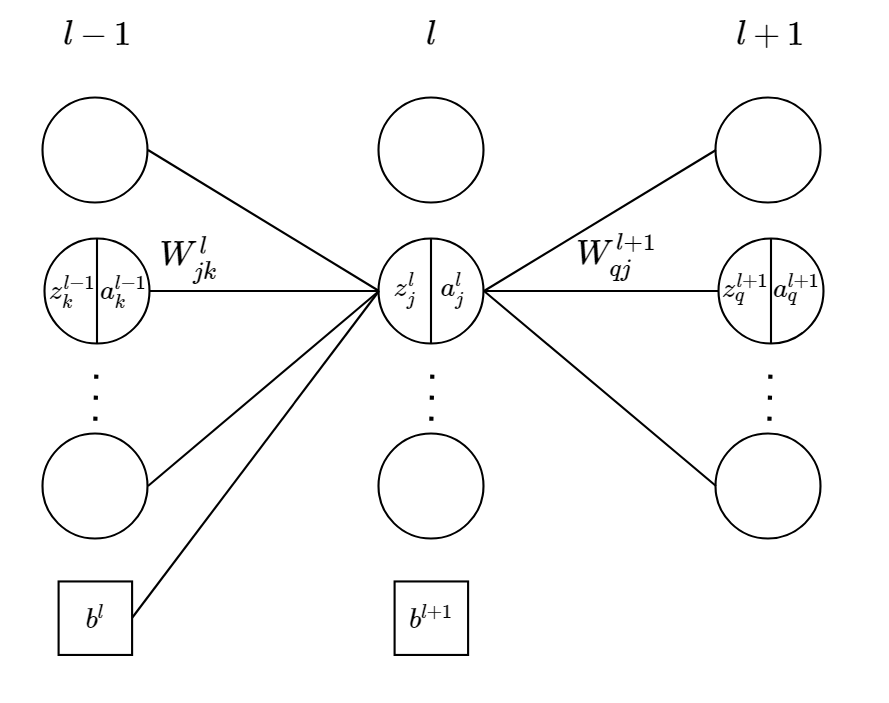
\includegraphics[width=0.6\textwidth]{images/backprop}
	\caption{Model of the neural network loss function with weights $W$, biases $b$, linearities $z$ and activations $a$ displayed at some layer $l$.}
	\label{fig:backprop}
\end{figure}

What remains is to compute the last terms of the equations \ref{eq:backprop_chainrule}. Since $\frac{\partial z^l_j}{\partial W^l_{jk}} = a^{l-1}_k$ and $\frac{\partial z^l_j}{\partial b_j^l} = 1$ we get

\begin{equation}
	\begin{aligned}
		\frac{\partial E(W_{jk}^l)}{\partial W_{jk}^l} &= \delta^l_j a^{l-1}_k, \\
		\frac{\partial E(b_j^l)}{\partial b_j^l} &= \delta^l_j.
	\end{aligned}
\end{equation}

Special care needs to be taken at the last layer of the network. Since it is usual to have only a linear layer at the end of a network without activation function the error variable (omitting the constants in the loss function) becomes 

\begin{equation}
	\begin{aligned}
		\delta^L = \frac{\partial L(z^L)}{\partial z^L} = \nabla L^T.
	\end{aligned}
\end{equation}

To efficiently implement backpropagation we can directly derive a matrix formulation so the iteration over all sample points is not required. By reformulating the loss function as $L(f(W;X),Y)$ with $X \in \R^{d \times N}, Y \in \R^{c \times N}, L: (\R^{c \times N},\R^{c \times N}) \to \R$, sample dimension $d$ and output dimension $c$ the activations and linearities are now matrices. To calculate the derivatives the involved matrices are vectorized in column-major order. Working through the stated derivation again but with the vectorized matrices we can rewrite the expressions in matrix form as

\begin{equation}
	\begin{aligned}
		\delta^l_m &= \delta^{l+1}_m W^{l+1} h'(z^l) = \delta^{l+1}_m W^{l+1} \odot H'(z^l)^T, \\
		\delta^L_m &= \text{reshape}(\frac{\partial L(z^L)}{\partial z^L}) = L_m, \\
		D_W^l &= \text{reshape}(\delta^l J^l), \\
		D_b^l &= \sum_{i=1}^{N} (\delta^l_m)_{i}^T.
	\end{aligned}
\end{equation}

The gradients are represented by $\nabla_{W^l}E = D^l_W$ and $\nabla_{b^l}E = D^l_b$. Each row in the matrix $L_m$ is the transpose gradient w.r.t. each sample point $\nabla L(z^L_i)$. Each row of the matrix $H'$ is the derivative of the activation function applied element wise to the each sample point. For $D^l_b$ the summation is over the rows $i$ of the matrix $\delta^l_m$. Note that $D^l_W$ can be implemented faster using per element multiplication but is written in full matrix form for easier reading. The matrix $J^l$ is the Jacobian $\frac{\partial z^l}{\partial W^l}$ with $W^l$ in row-major or column-major vectorization. In this formulation the vector version of the error variable $\delta^l$ is used. The reshape function extracts the rows and columns accordingly to get the matrix form.

\section{Additional notes and todos}

\begin{itemize}
	\item Could add regularizer for the weights.
	\item Put in $L$ the groundtruth as constants.
\end{itemize}

{\small
  \bibliographystyle{ieee}
  \bibliography{references}
}

\end{document}

